
\section{Motivation}

Knowing your machine is a major advantage when trying to optimize high-performance scientific code. \iaca\ \cite{iaca} is a tool by Intel to analyze \emph{X86} machine code with respect to a specific microarchitecture. However, it has some drawbacks that often times prevent it from being useful in practice. The main reason is that it doesn't support the newest processors. \iaca\ $3.0$, which was released in late 2017, supports the \nth{4} (Haswell) to the \nth{6} (Skylake) generation of Intel core microarchitectures. Skylake was released in 2015. \iaca\ $2.3$ additionally supports the \nth{2} (Sandy Bridge) and the \nth{3} (Ivy Bridge) generation. So at the time of writing \iaca\ is about three years behind and further development remains unclear.\\
The second complication is that \iaca\ is closed source. Its user guide \cite{userguide} is the only documentation it has which provides little to no information about how it actually computes its output. As a result a user will often find himself wondering how its output fits the analyzed program.\\
In this work we present \suaca\ (Saarland University Architecture Code Analyzer), an open source alternative. It uses measurements provided by \cite{Andreas} which are parsed during runtime. This way a user does not rely on a software update of the tool as he can simply perform the measurements on his own, should we not already support his microarchitecture. Note that this is only possible with Intel architectures so far. At the time of writing \suaca\ supports all Intel core microarchitectures from the \nth{1} (Nehalem) to the \nth{8} (Coffee Lake) generation, except for the server variant of Skylake.
\newpage

\section{Intel's microarchitectures}



In order to understand some of our computations one also needs some basic knowledge about Intel's microarchitectures. They use the \emph{X86} instruction
% Define the layers to draw the diagram
\pgfdeclarelayer{background}
\pgfdeclarelayer{background1}
\pgfdeclarelayer{foreground}
\pgfsetlayers{background,background1,main,foreground}

% Define block styles
\tikzstyle{nodeStyle} = [draw, text width=6cm,  minimum height=1.75em, text centered]
\tikzstyle{port} = [draw, fill={rgb,255:red,135; green,220; blue,170}, text width=0.75cm, font=\fontsize{6}{7.2}\sffamily, text centered]
\tikzstyle{FU} = [draw, fill={rgb,255:red,212; green,170; blue,0}, text width=5.0em, font=\fontsize{6}{7.2}\sffamily, rotate=90, text centered]
\tikzstyle{arrow} = [draw, thick, color=black!80, font=\footnotesize\sffamily]

% Draw background
\newcommand{\background}[7]{%
    \begin{pgfonlayer}{background}
        % Left-top corner of the background rectangle
        \path (#1.west |- #2.north)+(-1,0.4) node (a1) {};
        % Right-bottom corner of the background rectangle
        \path (#3.east |- #4.south)+(+0.4,#5) node (a2) {};
        % Draw the background
        \path[fill=#6, draw=black!50]
        (a1) rectangle (a2);
        \path let \p{x}=(a1), \p{y}=($(a1)!0.5!(a2)$) in (\x{x}, \y{y})+(0.5,0) node (u1)[rotate=90]
        {#7};
\end{pgfonlayer}}

\begin{figure}
    \centering
    \resizebox{!}{0.8\textheight}{
    \begin{tikzpicture}[scale=0.8,transform shape,font=\fontsize{11}{13.2}\sffamily]
    % Draw diagram elements
    \path node (nIC) [nodeStyle, fill={rgb,255:red,249; green,177; blue,166}] {Instruction Cache};
    \path (nIC.south)+(0.0,-1.0) node (nFD) [nodeStyle, fill={rgb,255:red,171; green,204; blue,227}] {Instruction Fetch \& Decode};
    \path (nFD.south)+(0.0,-1.3) node (nReorder) [nodeStyle, fill={rgb,255:red,198; green,233; blue,175}] {Reorder Buffer};
    \path (nReorder.south)+(0.0,-1.0) node (nRS) [nodeStyle, fill={rgb,255:red,135; green,220; blue,170}] {Scheduler};
    \path (nRS.south)+(-2.5,0.0) node[anchor=north] (nPort0) [port] {Port 0};
    \path (nRS.south)+(-1.5,0.0) node[anchor=north] (nPort1) [port] {Port 1};
    \path (nRS.south)+(-0.5,0.0) node[anchor=north] (nPort2) [port] {Port 2};
    \path (nRS.south)+(0.5,0.0) node[anchor=north] (nPort3) [port] {Port 3};
    \path (nRS.south)+(1.5,0.0) node[anchor=north] (nPort4) [port] {Port 4};
    \path (nRS.south)+(2.5,0.0) node[anchor=north] (nPort5) [port] {Port 5};
    
    \path (nPort0.south)+(0,-0.75) node[anchor=east] (nPort0FU) [FU] {ALU, V-MUL, \dots};
    \path (nPort1.south)+(0,-0.75) node[anchor=east] (nPort1FU) [FU] {ALU, V-ADD, \dots};
    \path (nPort2.south)+(0,-0.75) node[anchor=east] (nPort2FU) [FU] {Load, AGU};
    \path (nPort3.south)+(0,-0.75) node[anchor=east] (nPort3FU) [FU] {Load, AGU};
    \path (nPort4.south)+(0,-0.75) node[anchor=east] (nPort4FU) [FU] {Store Data};
    \path (nPort5.south)+(0,-0.75) node[anchor=east] (nPort5FU) [FU] {ALU, JMP, \dots};
    
    \begin{pgfonlayer}{background1}
    \path (nPort0FU.north |- nPort0FU.east)+(-0.25,0.25) node (ee_tl) {};
    \path (nPort5FU.south |- nPort5FU.west)+(+0.25,-0.25) node (ee_br) {};
    \path[fill={rgb,255:red,95; green,211; blue,188}, draw=black!50, rounded corners] (ee_tl) rectangle (ee_br);
    \end{pgfonlayer}
    
    \path let \p{x}=(nRS.south), \p{y}=(ee_br.south) in (\x{x}, \y{y})+(0,-1.0) node (nL1D)
    [nodeStyle, fill={rgb,255:red,249; green,177; blue,166}] {L1 Data Cache};
    \path (nL1D.south)+(0.0,-1.0) node (nL2) [nodeStyle, fill={rgb,255:red,249; green,177; blue,166}] {L2 Cache};
    
    % Draw arrows between elements
    \draw [->, arrow] (nIC.south) -- (nFD.north);
    \draw [->, arrow] (nFD.south) -- node [right] {4--6 \textnormal\microops} +(0,-0.6) -- (nReorder.north);
    \draw [->, arrow] (nReorder.south) -- node [right] {\textnormal\microops} (nRS.north);
    
    \draw [->, arrow, font=\fontsize{6}{7.2}\sffamily] (nPort0.south) -- node [right] {\textnormal\microop} +(-0,-0.5) -- (nPort0FU.east);
    \draw [->, arrow, font=\fontsize{6}{7.2}\sffamily] (nPort1.south) -- node [right] {\textnormal\microop} +(-0,-0.5) -- (nPort1FU.east);
    \draw [->, arrow, font=\fontsize{6}{7.2}\sffamily] (nPort2.south) -- node [right] {\textnormal\microop} +(-0,-0.5) -- (nPort2FU.east);
    \draw [->, arrow, font=\fontsize{6}{7.2}\sffamily] (nPort3.south) -- node [right] {\textnormal\microop} +(-0,-0.5) -- (nPort3FU.east);
    \draw [->, arrow, font=\fontsize{6}{7.2}\sffamily] (nPort4.south) -- node [right] {\textnormal\microop} +(-0,-0.5) -- (nPort4FU.east);
    \draw [->, arrow, font=\fontsize{6}{7.2}\sffamily] (nPort5.south) -- node [right] {\textnormal\microop} +(-0,-0.5) -- (nPort5FU.east);
    
    \draw [<->, arrow] (nPort2FU.west) -- (nPort2FU.west |- nL1D.north);
    \draw [<->, arrow] (nPort3FU.west) -- (nPort3FU.west |- nL1D.north);
    \draw [->, arrow] (nPort4FU.west) -- (nPort4FU.west |- nL1D.north);
    
    \draw [<->, arrow] (nL1D.south) -- (nL2.north);
    \draw [->, arrow] (nL2.east) -- +(+0.8,-0.0) |- (nIC.east);
    
    \background{nIC}{nIC}{nL2}{nFD}{-0.7}{{rgb,255:red,255; green,246; blue,213}}{Front End}
    \background{nReorder}{nReorder}{nL2}{ee_br}{-0.5}{{rgb,255:red,213; green,255; blue,230}}{Execution Engine}
    \background{nL1D}{nL1D}{nL1D}{nL2}{-0.4}{{rgb,255:red,252; green,222; blue,212}}{Memory}
    \end{tikzpicture}}
    \caption{Pipeline of Intel Core CPUs (simplified).}
\end{figure}

set. However, they don't execute those instructions directly. They will translate them into a sequence of so called \microops, which can then be executed. Unfortunately, there is little to no official documentation about those \microops, neither about the functionality of an individual one nor about their interaction with each other. From the measurements we can conclude that each microarchitecture has its own \microops\ which makes it even harder to find reliable information.\\ \autoref{fig:Pipeline} shows a sketch of a microarchitecture by Intel. We can see the front end including the decoder unit which is responsible for the translation of the instructions into the \microops. In our simulation we will only consider the number of \microops\ the front end produces each cycle, which is currently $4$--$6$ depending on the architecture. Our main interest lies in the execution engine or more precisely in the scheduler (or reservation station) and the ports. The scheduler is responsible for the distribution of the \microops\ over the ports. As mentioned before, a certain amount of those will be loaded into it by the frond end in each cycle. It has a maximum capacity, which also depends on the specific architecture (the scheduler of the Sandy Bridge architecture we will be using for most of our examples has a capacity of $54$). The most important property we can observe from this figure are the ports. Each port can be seen as a pipeline that a \microop\ can run through in order to be executed. On the ports themselves lie the actual execution units of the processor like the \emph{ALU}, \emph{MULTIPLEXER} and so on. Every port can hold a single \microop\ per cycle and they support pipelining. So they will be free again in the next cycle. The only exception from this is the \emph{DIVIDER} unit which is slow at executing and can be blocked for multiple cycles. Usually it is not necessary that the \microops\ are executed in program order. The so called out-of-order execution is possible whenever there is no dependency between the respective \emph{X86} instructions or the \microops\ themselves.
 
 %\begin{wrapfigure}[25]{l}{0.6\textwidth}
 %   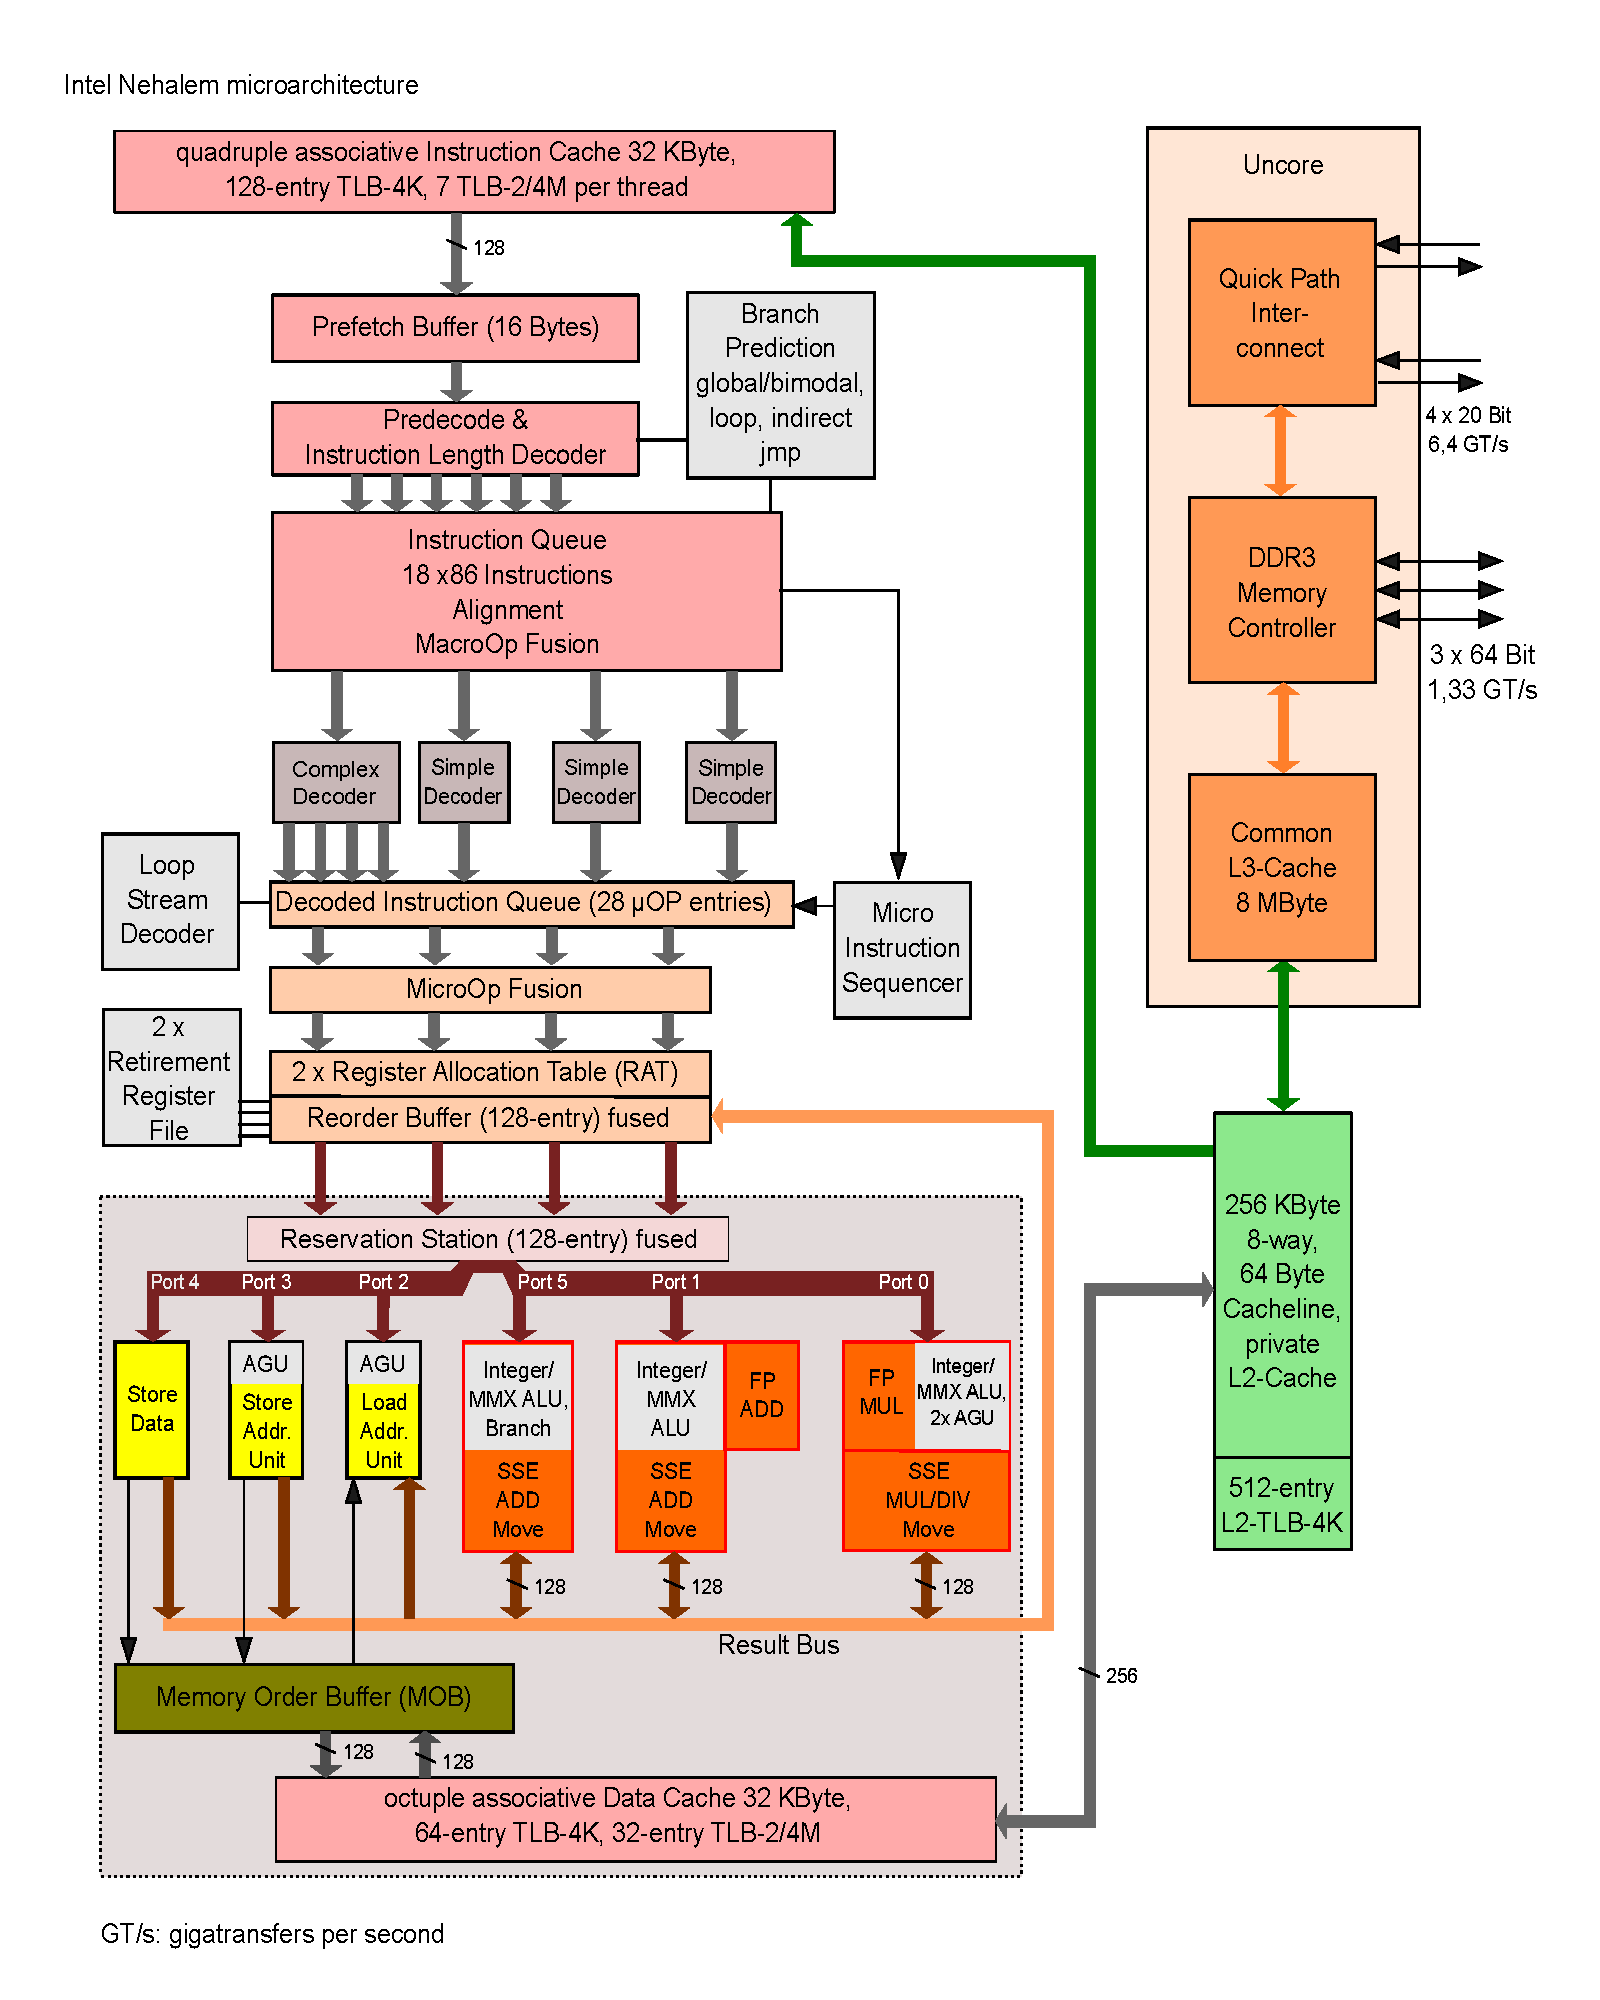
\includegraphics[width=0.6\textwidth]{Intel_Nehalem_arch}
 %  \caption{Intel Nehalem architecture \cite{nehalem}}
 % \label{fig:NHMfull}
 %\end{wrapfigure}
 
 
 %\begin{wrapfigure}[15]{r}{0.6\textwidth}
 %  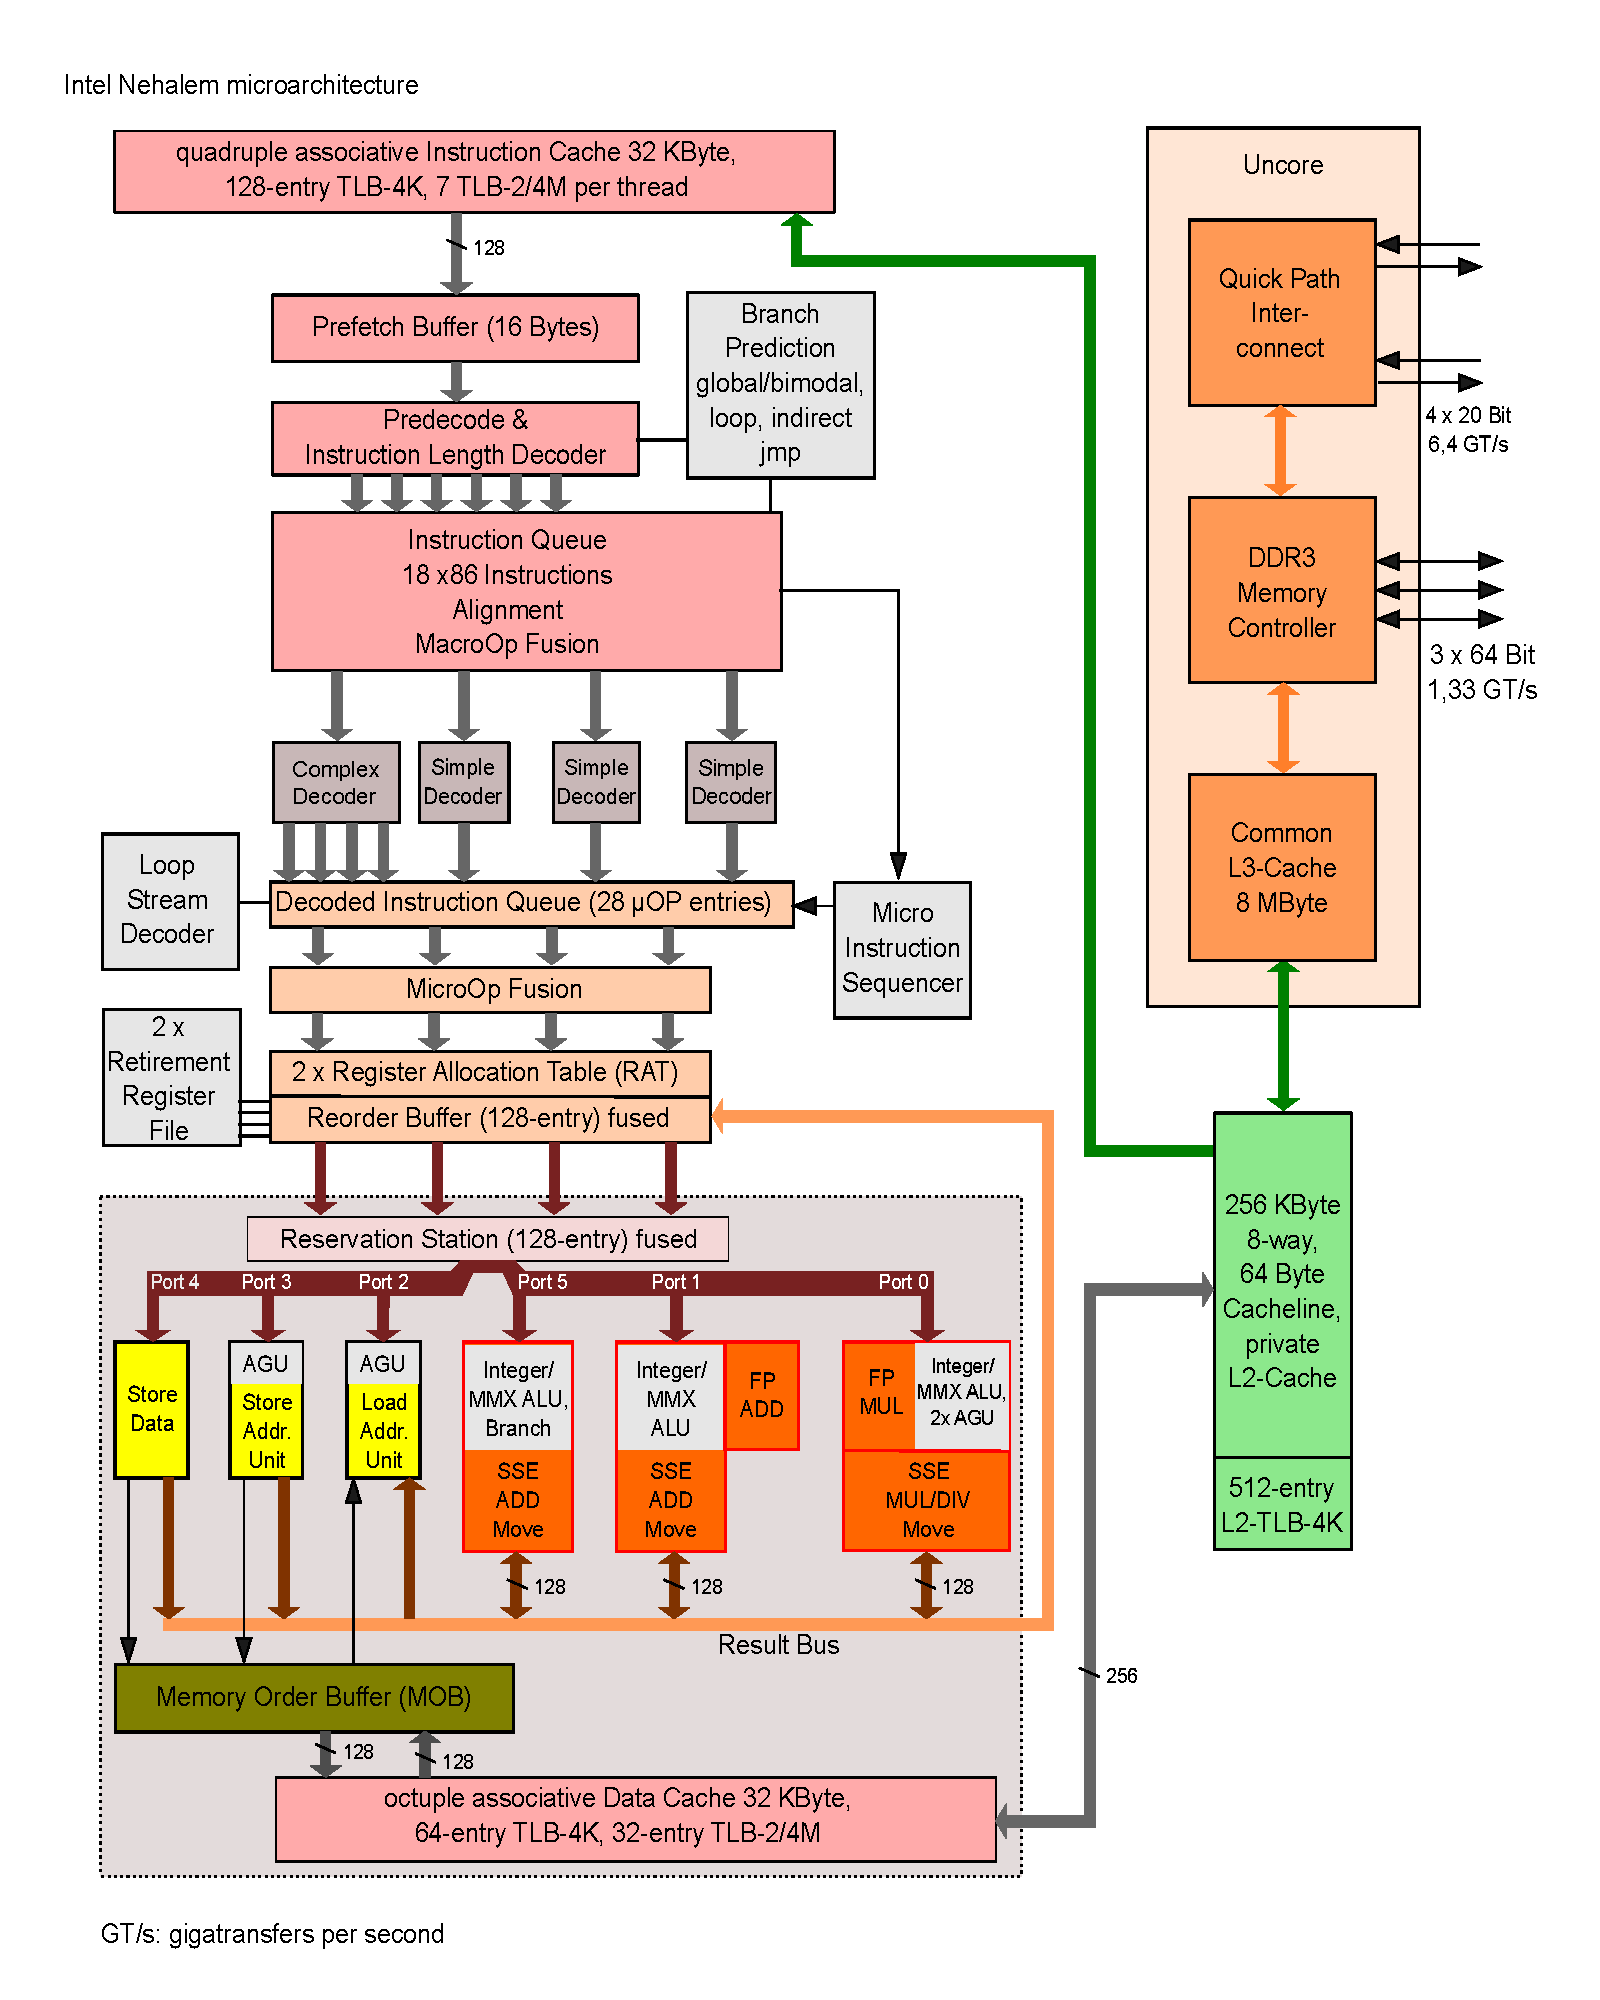
\includegraphics[clip, trim=0.5cm 2cm 9.78cm 20cm,width=0.6\textwidth]{Intel_Nehalem_arch}
 %\caption{Detailed view \cite{nehalem}}
 %\label{fig:NHMdetail}
 %\end{wrapfigure}
 
\section{\iaca's analysis} 
 \textbf{TODO}
 
 
\section{Scope of work}

Like mentioned before we will present a tool that is able to analyze \emph{X86} assembler code with respect to a specific microarchitecture. Just like \iaca\ our tool is able to find byte markers inside a compiled file and analyze the code in between. Those markers can be inserted in two different ways: inserting them by hand in the assembler code or use the \emph{iacaMarks.h} header in your \emph{C} code. First take a look at the assembly variant:

\begin{mdframed}[backgroundcolor=light-gray, roundcorner=10pt,leftmargin=1, rightmargin=1, innerleftmargin=15, innertopmargin=1,innerbottommargin=1, outerlinewidth=1, linecolor=light-gray]
    \begin{lstlisting}[language={myLang}]
    movl $111, %ebx
    .byte 0x64, 0x67, 0x90
    
    //Some code here
    
    movl $222, %ebx
    .byte 0x64, 0x67, 0x90
    \end{lstlisting}
\end{mdframed}

\iaca\ is mainly used to analyze critical parts of scientific code, which are usually inside a loop. When using a loop in \emph{C} code one can easily insert the markers defined in the \emph{iacaMarks.h} header like this:

\begin{mdframed}[backgroundcolor=light-gray, roundcorner=10pt,leftmargin=1, rightmargin=1, innerleftmargin=15, innertopmargin=1,innerbottommargin=1, outerlinewidth=1, linecolor=light-gray]
    \begin{lstlisting}
    #include "iacaMarks.h"
    
    int main(void) {
    
    while (condition) {
    (*@\textcolor{Green}{IACA\_START}  @*)
    //Some code here
    }
    (*@\textcolor{Green}{IACA\_END}  @*)
    
    return 0;
    }
    \end{lstlisting}
\end{mdframed}

In both cases a user has to compile his code and run \suaca\ on the compiled file. We are using Intel's \emph{X86 Encoder Decoder} library \cite{xed} to disassemble said file, which allows us to support files of the \emph{ELF}, \emph{PECOFF} and \emph{MACHO} format.\\
After disassembling \suaca\ will perform a dependency analysis on the instructions and parse the measurement file. Finally it will perform a simulation of the code. It won't consider the actual effect of the instructions, only their latencies, dependencies and port usage. The instructions are first considered in program order, although instruction reordering is still possible as we will see in \autoref{sec:chooseport}. For several reasons, which we will discuss in the following, our simulation will compute an estimate of the code's performance, not total numbers.\\
\suaca\ is able to perform several kinds of analyses which we will discuss in \autoref{chap:functionality}. In \autoref{chap:algorithms} we will then explain in detail how the most important parts of the simulation and the dependency analyzes are implemented.


\section{Measurements}
\label{sec:measurements}

As mentioned before a crucial part of \suaca's functionality are the measurements provided by \cite{Andreas}. Consider this snippet from the XML-measurement-file file:


\begin{lstlisting}[language=XML, basicstyle=\ttfamily\scriptsize, breaklines=false]
<instruction ... iform="ADD_LOCK_MEMv_GPRv" ...>
    <operand idx="2" type="reg" ...>RAX,RCX,RDX,RBX,...</operand>
    <operand idx="3" type="flag" ...>OF</operand>
    <operand idx="4" type="flag" ...>SF</operand>
    ...
    <architecture name="NHM">
        <measurement port15="2" port2="1" port3="1" port4="1" total_uops="5">
            <latency cycles="19" ... targetOp="3"/>
            <latency cycles="19" ... targetOp="4">
            ...
        <\measurement>
    </architecture>
<\instruction>
\end{lstlisting}

We dotted out some unnecessary or redundant information. As we can see in the first line this is the information for the instruction with the \emph{iform} ``ADD\_LOCK\_MEMv\_GPR''. \emph{iform} is an enum from the XED Library (\cite{xed}) that is used to identify instructions. We can extract the following information from our snippet:

\begin{itemize}
    \item One of the \emph{RAX, RCX, RDX, \dots} registers is an operand and they have the id $2$. We only need the mapping of $id \rightarrow register$ here as the xed library will tell us which operands are actually used in the analyzed programs. Similarly the flags also have their ids. The flags are the single bits of the \emph{RFLAGS} register in \emph{X86}.
    \item We have some measurements for the Intel Nehalem microarchitecture.
    \item When simulating Nehalem the instruction consists of $5$ \microops. Two of which can use ports $1$ and $5$ and one each can use port $2$, $3$ and $4$.
    \item It will take $19$ cycles to compute the result for the operand with id $3$.
\end{itemize}

Most instructions have several latency items, depending on the number and kind of operands. In our case there is no information for operand $2$ as the instruction won't write to those registers. However, the latency for the operand with id $4$ is also $19$ cycles. Some instructions actually produce their results in a specific order. It might be that one operand is available after $3$ cycles and another one after $5$, so an instruction that only needs the first of those operands has to wait $3$ cycles whereas another one that needs the second operand has to wait $5$. \suaca\ can simulate this behavior as it knows which operand is causing the dependency. When simulating the whole instruction \suaca\ takes the maximum of those values. Note that those values are always best case i.e., no port was blocked and no dependency occurred.\\
We can already observe why the lack of information on the \microops\ pose a major problem. We cannot know how the the above mentioned latency values come about. Probably those early results are computed by some of the \microops, but as we do not know which ones we can not always precisely compute the correct latency should an instruction be delayed. If the \microops\ of an instruction do not depend on each other it is even possible that the order of the results changes, which we also can not simulate.
%TODO last paragraph is questionable

\section{Related work}

Like mentioned before one can find general information about \iaca\ at its website \cite{iaca}. The user's guide \cite{userguide} gives additional information about the usage and provides some examples. \iaca\ is developed by Israel Hirsh and Gideon~S.\\

Andreas Abel \cite{Andreas} provides the measurements which enable us to compute our results.\\

Jan Laukemann \cite{osaca-thesis} implemented an open source alternative to \iaca\ called \osaca\ \cite{osaca-web}. It relies on the measurements provided by Johannes Hofmann \cite{ibench}. We will discuss the difference between the three tools in \autoref{chap:eval}.
